\documentclass[tikz]{standalone}
\usepackage{helvet}
\usepackage[T1]{sansmath}
\renewcommand{\familydefault}{\sfdefault}
\normalfont

\begin{document}
\begin{sansmath}


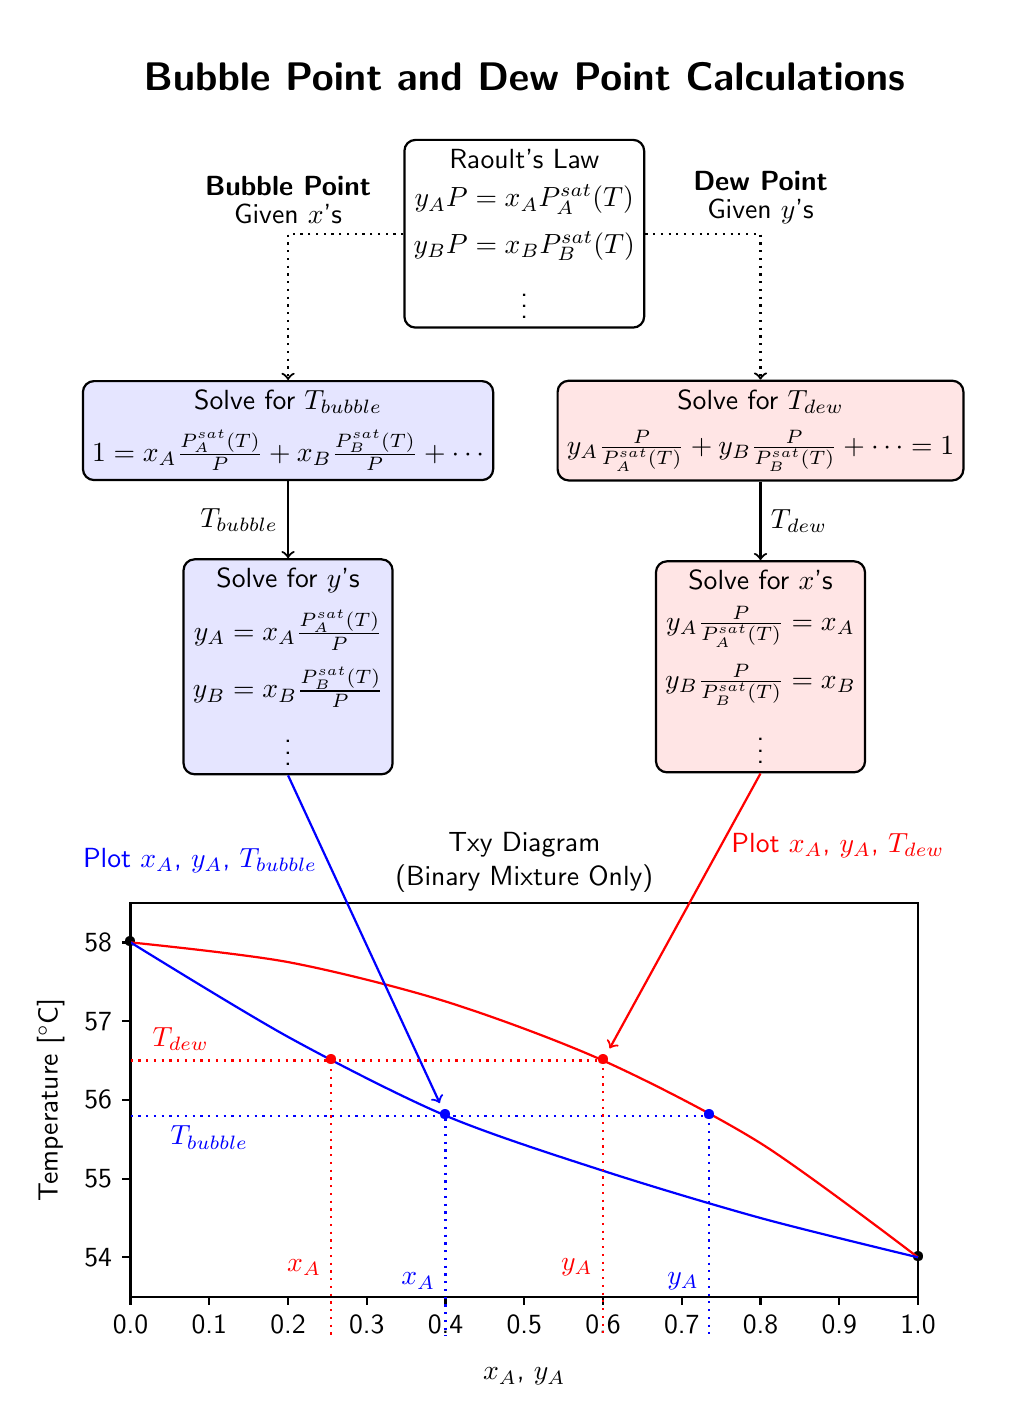
\begin{tikzpicture}[auto,thick]
    %\draw[help lines] (0,1) grid (12,21);
    \node at (12,19.5) {};
    
    \node[rectangle] (title) at (6,19)
    	{\Large \bf Bubble Point and Dew Point Calculations};
    
    \node[rectangle,draw, rounded corners] (tbox1) at (6,17)
    	{\shortstack{Raoult's Law \\ \\
    		$y_A P = x_A P^{sat}_A(T)$\\ \\
    		$y_B P = x_B P^{sat}_B(T)$\\ \\
    		$\vdots$}};

    \node[rectangle,draw, rounded corners, fill=blue!10] 
    	(tbox4) at (3.0,11.5) 
    	{\shortstack{Solve for $y$'s\\ \\
    		$y_A = x_A \frac{P^{sat}_A(T)}{P}$\\ \\
    		$y_B = x_B \frac{P^{sat}_B(T)}{P}$\\ \\
    		$\vdots$}};

    \node[rectangle,draw, rounded corners, fill=red!10]
    	(tbox5) at (9.0,11.5)
    	{\shortstack{Solve for $x$'s\\ \\
    		$y_A \frac{P}{P^{sat}_A(T)} = x_A$\\ \\
    		$y_B \frac{P}{P^{sat}_B(T)} = x_B$\\ \\
    		$\vdots$}};
    	
    \node[rectangle,draw, rounded corners, fill=blue!10]
    	(tbox2) at (3.0,14.5)
    	{\shortstack{Solve for $T_{bubble}$ \\ \\
    		$1 = x_A \frac{P^{sat}_A(T)}{P} + x_B \frac{P^{sat}_B(T)}{P} + \cdots$}};

    \node[rectangle,draw, rounded corners, fill=red!10]
    	(tbox3) at (9.0,14.5)
    	{\shortstack{Solve for $T_{dew}$ \\ \\
    		$y_A \frac{P}{P^{sat}_A(T)} + y_B \frac{P}{P^{sat}_B(T)} + \cdots = 1$}};
    	
   	\draw[->,dotted] (tbox1) --++(-3.0,0)
    	node[above] {\shortstack{{\bf Bubble Point}\\Given $x$'s}}
    	-- (tbox2.north);
    	
    \draw[->,dotted] (tbox1) --++(3.0,0)
    	node[above] {\shortstack{{\bf Dew Point}\\Given $y$'s}}
    	-- (tbox3.north);

    \draw[->] (tbox2.south) -- (tbox4.north)
    	node[left,midway] {$T_{bubble}$};

    \draw[->] (tbox3.south) -- (tbox5.north)
    	node[right,midway] {$T_{dew}$}  ;

    \node[rectangle,draw,minimum height = 5cm, minimum width = 10cm]
    	(Txy) at (6,6) {};
     
    \node at (1,8) {\textbullet};
    \node at (11,4) {\textbullet};
    \draw [red] plot [smooth] coordinates 
    	{(1,8) (3,7.75) (5,7.25) (7,6.5) (9,5.45) (11,4)};
    \draw [blue] plot [smooth] coordinates 
    	{(1,8) (3,6.8) (5,5.8) (7,5.1) (9,4.5) (11,4)};
    \foreach \x in {0,...,9}
     	\draw (\x,3.5)++(1,0) -- ++(0,-3pt)
			node[anchor=north] {0.\x};
    \foreach \x in {4,...,8}
     	\draw (1,\x) -- ++(-3pt,0)
			node[anchor=east] {5\x};
	\draw (8,3.5)++(3,0) -- ++(0,-3pt) node[anchor=north] {1.0};
	\draw (Txy.south)++(0,-1) node {$x_A$, $y_A$};
    \draw (Txy.west)++(-1.0,0) 
    	node [rotate=90] {Temperature [$^\circ$C]};
    \draw (Txy.north)++(0,0.5) 
    	node {\shortstack{Txy Diagram\\(Binary Mixture Only)}};
     
    \node[blue] at (5,5.8) {\textbullet};
    \node[blue] at (8.35,5.8) {\textbullet};
    \draw[->,blue,shorten >= 5pt] (tbox4.south) -- (5,5.8)
    	node[near start,left] {Plot $x_A$, $y_A$, $T_{bubble}$};
    \draw[blue,dotted] (1,5.8) -- (5,5.8)
    	node[below,near start] {$T_{bubble}$} -- (5,3)
    	node[left,near end] {$x_A$};
    \draw[blue,dotted] (5,5.8) -- (8.35,5.8) -- (8.35,3)
    	node[left,near end] {$y_A$};
    
    \node[red] at (7,6.5) {\textbullet};
    \node[red] at (3.55,6.5) {\textbullet};
    \draw[->,red,shorten >= 5pt] (tbox5.south) -- (7,6.5)
    	node[right,near start] {Plot $x_A$, $y_A$, $T_{dew}$};
    \draw[red,dotted] (1,6.5) -- (3.55,6.5)
    	node[above,near start] {$T_{dew}$} -- (3.55,3)
    	node[left,near end] {$x_A$};
    \draw[red,dotted] (3.55,6.5) -- (7,6.5) -- (7,3)
    	node[left,near end] {$y_A$};

\end{tikzpicture}

\end{sansmath}
\end{document}
